% !TEX root = MAIN.tex


\section{DAMTE}

\begin{figure}[]
  \centering
	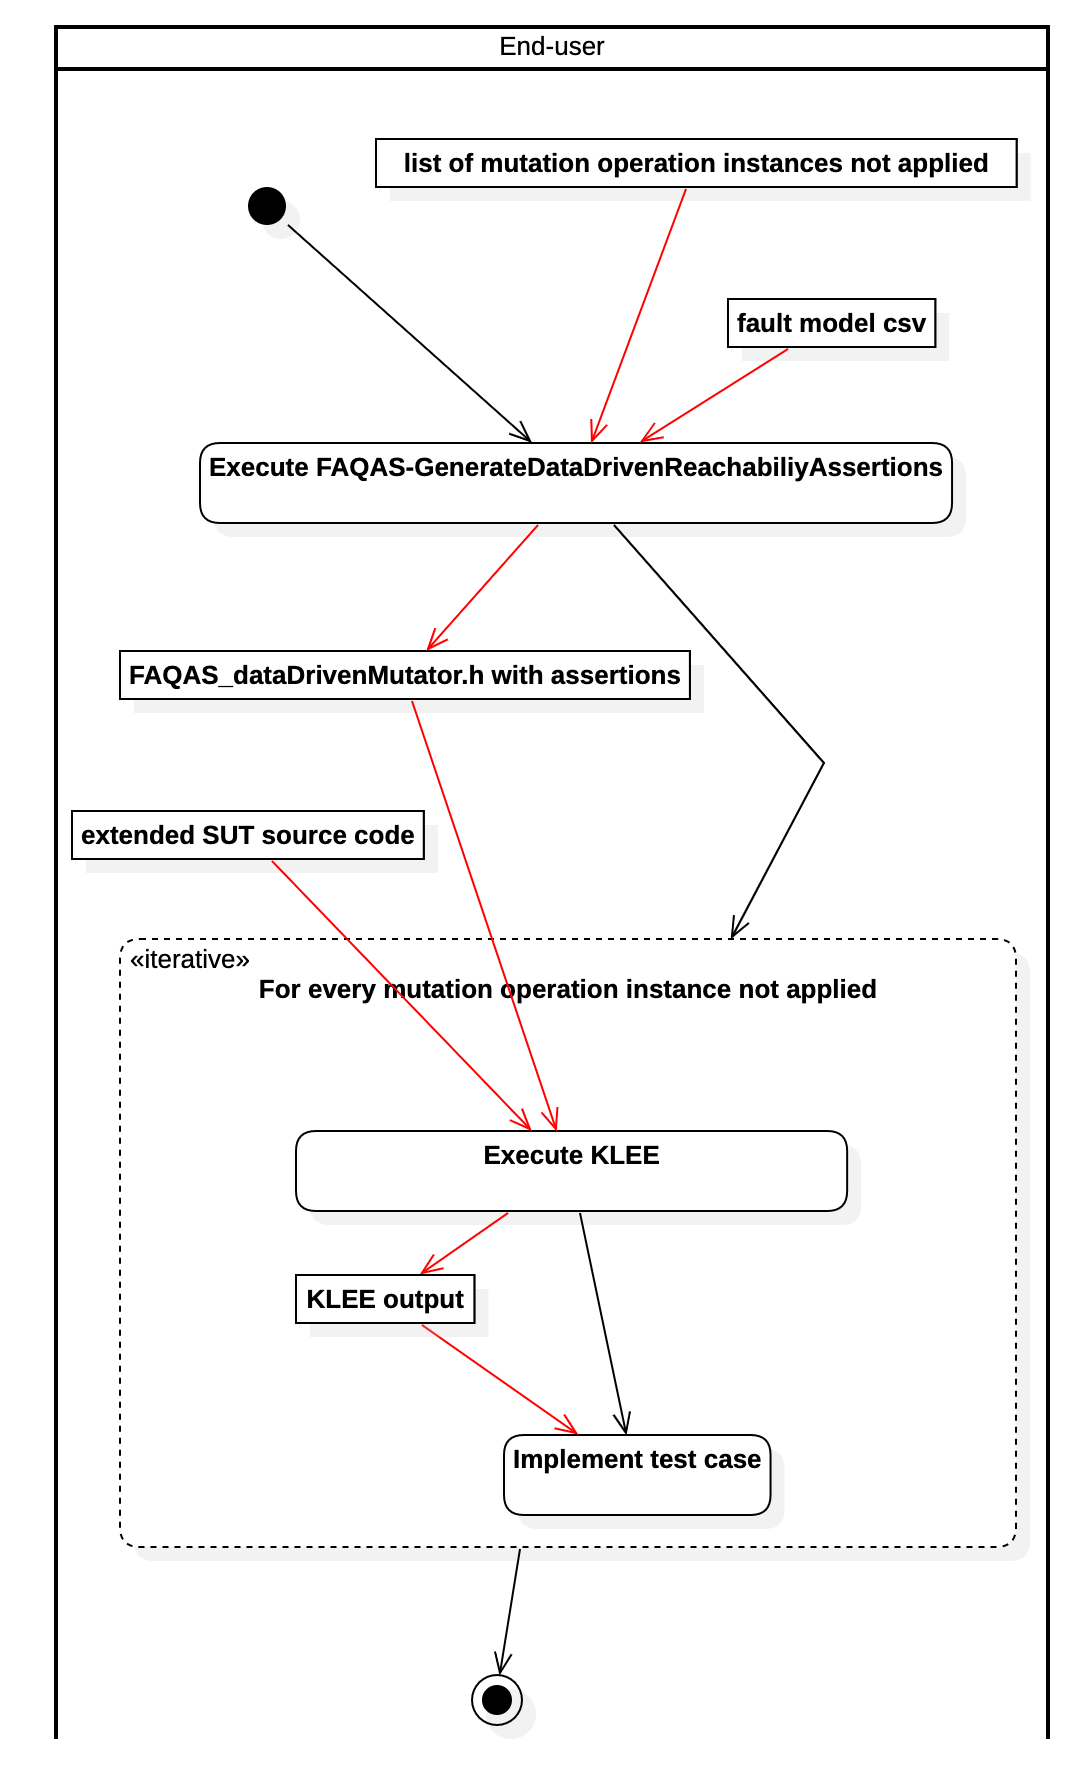
\includegraphics[width=0.4\textwidth]{images/png/Activity1!DataDrivenTestSuiteAugmentation_4.png}
      \caption{Overview of the data-driven test suite augmentation process.}
      \label{fig:process:dataDriven:augment}
\end{figure}

The activity \emph{Execute FAQAS-GenerateDataDrivenReachabiliyAssertions} in Figure~\ref{fig:process:dataDriven:augment} concerns the execution of the program \emph{Execute FAQAS-GenerateDataDrivenReachabiliyAssertions}.

The program \emph{FAQAS-GenerateDataDrivenReachabiliyAssertions} takes as input the fault model and generates a version of \emph{FAQAS\_dataDrivenMutator.h} that contains reachability assertions that enable KLEE to generate inputs that reach the mutation.

The activity \emph{Execute KLEE} indicates that the end-user should execute KLEE, after performing the required scaffolding, if necessary. A methodological procedure document to support the end-user will be provided.

The activity \emph{Implement test case} indicates that the end-user should implement a test case based on KLEE's output.

